\documentclass[11pt,letterpaper]{article}
\usepackage[margin=.90in]{geometry}
\usepackage[T1]{fontenc}
\usepackage[utf8]{inputenc}
\usepackage{lmodern,microtype}
\usepackage{amsmath,amssymb,amsthm,mathtools}
\usepackage{tikz}
\usetikzlibrary{arrows.meta,positioning,calc,fit,decorations.pathreplacing}
\usepackage{booktabs,enumitem,tabularx}
\usepackage{hyperref}
\hypersetup{colorlinks=true,linkcolor=blue!55!black,citecolor=blue!55!black,urlcolor=blue!55!black,pdftitle={Contractible Carriers and Null Attachments in Clique Complexes}}
\usepackage{caption}
\newtheorem{theorem}{Theorem}[section]
\newtheorem{proposition}[theorem]{Proposition}
\newtheorem{lemma}[theorem]{Lemma}
\newtheorem{corollary}[theorem]{Corollary}
\theoremstyle{definition}
\newtheorem{example}[theorem]{Example}
\newtheorem{definition}[theorem]{Definition}
\theoremstyle{remark}
\newtheorem{remark}[theorem]{Remark}
\newcommand{\Del}{\Delta}
\newcommand{\Star}{\operatorname{st}}
\newcommand{\Link}{\operatorname{lk}}
\newcommand{\SigmaU}{\Sigma_{\mathrm u}}
\newcommand{\N}{N}
\definecolor{darkblue}{RGB}{29,60,91}
\definecolor{tealblue}{RGB}{43,125,145}
\definecolor{redorange}{RGB}{199,112,44}
\definecolor{lightgray}{RGB}{241,246,249}
\tikzset{vtx/.style={circle,draw=darkblue,line width=.8pt,fill=white,inner sep=1.2pt,minimum size=5.8mm,font=\scriptsize},
  gedge/.style={draw=darkblue,line width=.95pt},
  target/.style={draw=tealblue,line width=1.4pt},
  source/.style={draw=redorange,line width=1.15pt},
  foldarrow/.style={-{Latex[length=1.7mm]},draw=tealblue,dashed,line width=.9pt},
  steparrow/.style={-{Latex[length=2.7mm]},draw=darkblue,line width=1.1pt}}
\title{\textbf{Contractible Carriers and Null Attachments}\\[5pt]
\large A certified extension of the vertex-star homotopy-cofiber method}
\author{Research note on clique complexes and graph folds}
\date{13 November 2026}
\begin{document}
\maketitle
\begin{abstract}
Deleting a vertex from a finite graph separates its clique complex into a deletion and the cone over its open-neighborhood complex.  The resulting homotopy type depends on the attaching map.  We establish a certificate for null-homotopy that requires neither a dimension inequality nor a cone point: after ordinary dominated-vertex folds of the deletion, it suffices that the full image of the link lie in a contractible simplicial subcomplex.  We prove this criterion carefully, show how an independent sequence of graph \(s\)-dismantlings certifies the carrier's contractibility, and work through small examples with TikZ diagrams.  A fully specified 15-vertex graph illustrates a nonconical four-vertex path carrier; its clique complex is \(S^1\vee S^2\).  We distinguish this fixed-fold certificate from the stronger claim that no alternative cone-image certificate exists, and describe bounded, replayable computational verification.
\end{abstract}
\tableofcontents

\section{Simplicial conventions and the cofiber}
All graphs are finite, simple, and undirected. A \emph{complete} is a nonempty set of pairwise adjacent vertices. A \emph{clique} is an inclusion-maximal complete. The \emph{clique complex} \(\Del(H)\) is the simplicial complex of all completes of \(H\) (together with the empty face). In particular, a face need not be a maximal clique. For comparison, the \emph{clique graph} \(K(G)\) is the graph whose vertices are the maximal completes of \(G\), adjacent when they intersect. The arguments below concern \(\Del(H)\); they apply to a clique graph by setting \(H=K(G)\).

For a vertex \(v\), let \(H-v\) be its deletion, \(\N_H(v)\) its \emph{open} neighborhood, and \(H[\N_H(v)]\) the induced neighborhood graph. Set
\[
 B=\Del(H-v),\quad L=\Del(H[\N_H(v)]),\quad X=\Del(H).
\]
We always assume \(L\ne\varnothing\) and, for the wedge formulas below, that \(B\) is path-connected.

\begin{proposition}[Vertex-star identity]\label{prop:star}
There is a simplicial equality
\[
 \boxed{X=B\cup_L(v*L)}.
\]
Here \(v*L\) is the simplicial cone over \(L\). Its intersection with \(B\) is exactly \(L\), so the geometric realization of \(X\) is the mapping cone of the simplicial inclusion \(j:L\hookrightarrow B\).
\end{proposition}
\begin{proof}
Every complete of \(H\) either avoids \(v\), hence belongs to \(B\), or is \(\{v\}\cup\tau\), where every vertex of \(\tau\) belongs to \(\N_H(v)\) and \(\tau\) is a complete. In the latter case \(\tau\in L\). Conversely every face of the indicated union is a complete of \(H\). The common faces are precisely the faces not containing \(v\), namely \(L\). Realization of a simplicial cone is a topological cone, and all inclusions of subcomplexes are cofibrations. Thus the union is the usual mapping-cone model \cite[Ch.~0]{Hatcher2002}.
\end{proof}

\begin{figure}[htbp]
\centering
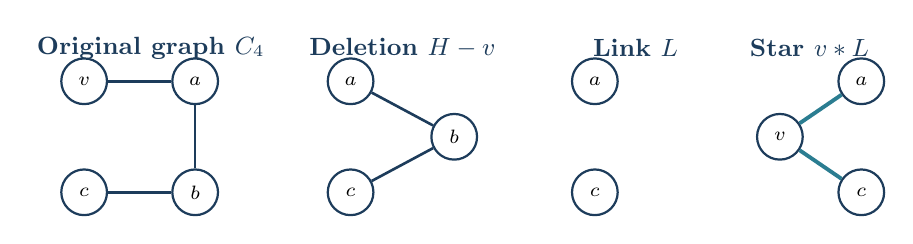
\begin{tikzpicture}[scale=.94]
\begin{scope}[shift={(-4.8,0)}]
\node[font=\small\bfseries, darkblue] at (.9,1.45) {Original graph \(C_4\)};
\node[vtx] (v) at (0,1) {\(v\)};
\node[vtx] (a) at (1.5,1) {\(a\)};
\node[vtx] (b) at (1.5,-.5) {\(b\)};
\node[vtx] (c) at (0,-.5) {\(c\)};
\draw[gedge] (v)--(a)--(b)--(c)--cycle;
\end{scope}
\begin{scope}[shift={(-1.2,0)}]
\node[font=\small\bfseries, darkblue] at (.7,1.45) {Deletion \(H-v\)};
\node[vtx] (aa) at (0,1) {\(a\)};
\node[vtx] (bb) at (1.4,.25) {\(b\)};
\node[vtx] (cc) at (0,-.5) {\(c\)};
\draw[gedge] (aa)--(bb)--(cc);
\end{scope}
\begin{scope}[shift={(2.1,0)}]
\node[font=\small\bfseries, darkblue] at (.55,1.45) {Link \(L\)};
\node[vtx] at (0,1) {\(a\)};
\node[vtx] at (0,-.5) {\(c\)};
\end{scope}
\begin{scope}[shift={(4.6,0)}]
\node[font=\small\bfseries, darkblue] at (.4,1.45) {Star \(v*L\)};
\node[vtx] (vv) at (0,.25) {\(v\)};
\node[vtx] (av) at (1.1,1) {\(a\)};
\node[vtx] (cv) at (1.1,-.5) {\(c\)};
\draw[target] (vv)--(av) (vv)--(cv);
\end{scope}
\end{tikzpicture}
\caption{The deletion plus the cone on the two-point link reconstructs \(\Del(C_4)\). The star and deletion meet along the link.}
\label{fig:pushout}
\end{figure}

For a nonempty CW complex \(L\), let \(\SigmaU L\) denote the \emph{unreduced} suspension: the two ends of \(L\times[0,1]\) are collapsed separately. This convention matters for disconnected links.

\begin{theorem}[Null-attachment splitting]\label{thm:split}
If \(j:L\to B\) is null-homotopic, then
\[
 \boxed{X\simeq B\vee\SigmaU L.}
\]
If \(L\) has \(r\ge1\) nonempty connected components \(L_i\), then
\[
 \SigmaU L\simeq\left(\bigvee_{i=1}^r\SigmaU L_i\right)\vee\bigvee^{r-1}S^1.
\]
\end{theorem}
\begin{proof}
The homotopy-cofiber is \(B\cup_j CL\). Replace \(j\) by a constant attaching map using the homotopy extension property of the CW pair \((CL,L)\): homotopic attachments yield homotopy-equivalent spaces \cite[Prop.~0.18]{Hatcher2002}. For a constant attachment, the cone base \(L\) is identified to a chosen point of \(B\), producing \(B\vee(CL/L)=B\vee\SigmaU L\).

For the disconnected formula, choose one arc between the two suspension poles for each component. The union of the \(r\) arcs is a graph with first Betti number \(r-1\). Each remaining connected suspension attaches to the arcs along a contractible CW subcomplex; collapsing these arcs is a homotopy equivalence \cite[Prop.~0.17 and Ch.~0, Exercise~25]{Hatcher2002}. This gives the displayed formula.
\end{proof}

\begin{example}[A square, and the importance of the link map]\label{ex:square}
Take \(H=C_4\) and \(v\) as in Figure~\ref{fig:pushout}. The deletion is a tree, hence contractible, and the link consists of two points (\(S^0\)). The attachment is null, so \(\Del(C_4)\simeq\SigmaU S^0\simeq S^1\). In contrast, if \(H\) is a four-cycle with an additional hub adjacent to all four cycle vertices, then for that hub \(B=L=\Del(C_4)\cong S^1\) and \(j\) is the identity. The star fills the cycle with a cone and \(\Del(H)\) is contractible, \emph{not} \(S^1\vee S^2\). Thus one cannot infer the cofiber from the abstract types of \(B\) and \(L\) alone.
\end{example}

\section{Ordinary graph folds and contractible carriers}
An \emph{ordinary graph fold} is the deletion of a vertex \(x\) dominated by a distinct adjacent vertex \(y\), meaning \(\N_D[x]\subseteq\N_D[y]\) for closed neighborhoods. This is different from the graph \(s\)-dismantling used below.

\begin{lemma}[Ordinary folds produce simplicial retractions]\label{lem:fold}
Suppose \(\N_D[x]\subseteq\N_D[y]\), \(x\ne y\). The vertex map sending \(x\) to \(y\) and fixing all other vertices induces a simplicial retraction \(p:\Del(D)\to\Del(D-x)\). Moreover \(p\) is a homotopy equivalence. A sequence of such folds therefore yields a simplicial homotopy equivalence \(r:\Del(D)\to\Del(D')\), with an explicit map on the original vertices.
\end{lemma}
\begin{proof}
If a complete \(\sigma\) contains \(x\), each other vertex of \(\sigma\) is adjacent to \(x\), hence to \(y\), and \(x\) itself is adjacent to \(y\). Consequently the image of \(\sigma\) under the vertex map is again a complete (repeated vertices are allowed in the image of a simplicial map). The inclusion \(\Del(D-x)\hookrightarrow\Del(D)\) is a right inverse. Furthermore, for each face \(\sigma\), the union of \(\sigma\) and the image of \(\sigma\) is a face. The two maps are therefore contiguous and induce homotopic maps on geometric realizations \cite[Chs.~2--3]{Kozlov2008}. Thus \(p\) and the inclusion are homotopy inverses. Iterating proves the statement.
\end{proof}

\begin{definition}[Contractible carrier]
For a simplicial map \(f:L\to\Del(D')\), a \emph{carrier} is a subcomplex \(A\subseteq\Del(D')\) that contains the entire image \(f(L)\). In the implementation considered here, \(A=\Del(D'[W])\) is the flag complex induced on a prescribed vertex set \(W\), so it suffices that \(W\) contain every image vertex. A \emph{contractible-carrier certificate} proves \(A\simeq\{\ast\}\), rather than only that its homology vanishes.
\end{definition}

\begin{theorem}[Contractible-carrier null-attachment criterion]\label{thm:carrier}
Let \(H\) be a finite graph, \(v\in V(H)\), and assume \(B=\Del(H-v)\) is nonempty and path-connected. Suppose ordinary graph folds of \(H-v\) yield a graph \(D'\), with induced simplicial homotopy equivalence \(r:B\to\Del(D')\). Let \(W\subseteq V(D')\) contain all images under \(r\) of vertices in \(\N_H(v)\). If \(\Del(D'[W])\) is contractible, then the link inclusion \(j:L\hookrightarrow B\) is null-homotopic. Consequently
\[
 \boxed{\Del(H)\simeq\Del(H-v)\vee\SigmaU\Del(H[\N_H(v)]).}
\]
No restriction on the dimensions of spheres occurring in \(L\) or \(B\) is needed.
\end{theorem}
\begin{proof}
Because \(r\) is a simplicial map and the image vertices of every face of \(L\) belong to \(W\), the composite \(r\circ j:L\to\Del(D')\) factors through \(A=\Del(D'[W])\). Contractibility of \(A\) implies that \(r\circ j\) is null-homotopic. Let \(s\) be a homotopy inverse of \(r\), furnished by Lemma~\ref{lem:fold}. Then \(j\simeq s\circ r\circ j\) is null-homotopic as well. Apply Theorem~\ref{thm:split}. \end{proof}

\begin{remark}[What is genuinely new?]\label{rem:notcone}
If \(W\) has a universal vertex in \(D'[W]\), then \(A\) is a simplicial cone and automatically contractible; this is the previously implemented \emph{cone-image} criterion. A contractible carrier can have \emph{no} universal vertex, as the path in Figure~\ref{fig:path} demonstrates. The extension is a relaxation at a \emph{specified folded target}. It does not imply that some other, longer ordinary-fold sequence could never produce a cone-image witness.
\end{remark}

\section{Certifying contractibility by s-dismantlings}
A vertex \(w\) of a graph \(A\) is \emph{\(s\)-dismantlable} if its open neighborhood \(A[\N_A(w)]\) is an ordinarily dismantlable nonempty graph, that is, it reduces to one vertex by successive dominated-vertex deletions. This graph-theoretic condition is related to simplicial simple-homotopy by Boulet--Fieux--Jouve \cite{BouletFieuxJouve2010}. We record the topological argument needed here.

\begin{proposition}[An \(s\)-dismantling preserves homotopy type]\label{prop:s}
If \(w\) is \(s\)-dismantlable in \(A\), then the natural inclusion \(\Del(A-w)\hookrightarrow\Del(A)\) is a homotopy equivalence. Hence an explicitly verified sequence of such moves reducing \(A\) to one vertex proves \(\Del(A)\) contractible.
\end{proposition}
\begin{proof}
By Lemma~\ref{lem:fold}, dismantling the open neighborhood proves that the link \(L_w=\Del(A[\N_A(w)])\) is contractible. Proposition~\ref{prop:star} gives \(\Del(A)=\Del(A-w)\cup_{L_w}(w*L_w)\). The inclusion \(L_w\hookrightarrow w*L_w\) is a homotopy equivalence because both spaces are contractible. Since \(L_w\hookrightarrow\Del(A-w)\) is a cofibration, the gluing lemma for homotopy pushouts gives a homotopy equivalence \(\Del(A-w)\simeq\Del(A)\); equivalently, use Theorem~\ref{thm:split} with a contractible link. Iterate. If the final graph is a singleton, its clique complex is a point.
\end{proof}

\begin{figure}[htbp]
\centering
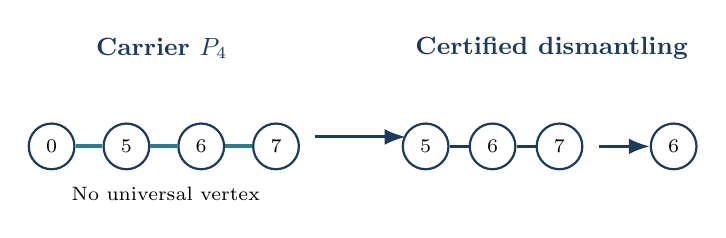
\begin{tikzpicture}[scale=1]
\begin{scope}[shift={(-3.5,0)}]
\node[font=\small\bfseries,darkblue] at (1.4,1.25) {Carrier \(P_4\)};
\node[vtx] (aa) at (0,0) {\(0\)};
\node[vtx] (bb) at (.95,0) {\(5\)};
\node[vtx] (cc) at (1.9,0) {\(6\)};
\node[vtx] (dd) at (2.85,0) {\(7\)};
\draw[target] (aa)--(bb)--(cc)--(dd);
\node[font=\scriptsize] at (1.45,-.6) {No universal vertex};
\end{scope}
\draw[steparrow] (-.15,.12)--(1,.12);
\begin{scope}[shift={(1.25,0)}]
\node[font=\small\bfseries,darkblue] at (1.6,1.25) {Certified dismantling};
\node[vtx] (bb) at (0,0) {\(5\)};
\node[vtx] (cc) at (.85,0) {\(6\)};
\node[vtx] (dd) at (1.7,0) {\(7\)};
\draw[gedge] (bb)--(cc)--(dd);
\draw[steparrow] (2.2,0)--(2.85,0);
\node[vtx] at (3.15,0) {\(6\)};
\end{scope}
\end{tikzpicture}
\caption{The induced image path \(P_4=0-5-6-7\) is contractible, although it is not a cone. Ordinary folds \(0\mapsto5\), \(7\mapsto6\), and \(5\mapsto6\) collapse it to one vertex (the schematic displays intermediate endpoints).}
\label{fig:path}
\end{figure}

\begin{remark}[Independent verification]
To check a carrier certificate, reconstruct the induced graph \(D'[W]\), then for each recorded removal of \(w\) independently verify every local closed-neighborhood domination in \(D'[W][\N(w)]\). Remove \(w\) only after its local proof passes; require a final single vertex. This is stronger than checking Betti numbers or an Euler characteristic. A certificate should fail closed if vertices or moves are missing, malformed, or exceed configured bounds.
\end{remark}

\section{Worked example: a nonconical image carrier}
\subsection{Complete graph specification}
We now give a self-contained 15-vertex example where both the deletion and the link have type \(S^1\), but the attaching map is null-homotopic for a \emph{certified} reason.

Let \(D_0\) have vertices \(0,\ldots,7\) and edges
\[
 E(D_0)=\{01,12,23,34,40,05,56,67\}.
\]
Thus \(D_0\) consists of a five-cycle and a path of three edges rooted at vertex \(0\). Define
\[
 (t_8,t_9,t_{10},t_{11},t_{12},t_{13})=(0,5,6,7,6,5).
\]
Create six further vertices \(8,\ldots,13\), add the six-cycle \(8-9-10-11-12-13-8\), and join each vertex \(i\in\{8,\ldots,13\}\) to \(t_i\) and every neighbor of \(t_i\) in \(D_0\). No other edges are added. Denote the resulting graph on 14 vertices by \(D\). Finally add a new vertex \(v=14\) adjacent \emph{only} to \(8,\ldots,13\), obtaining the graph \(H\). The construction has \(38\) edges and graph6 string \verb!NhEMKC@?KC|o^@M?~_?! (the labelled construction, rather than this optional encoding, fixes the graph unambiguously).

\begin{figure}[htbp]
\centering
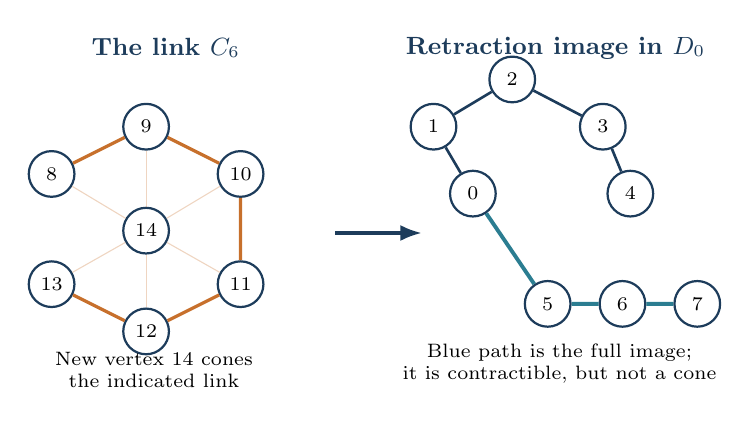
\begin{tikzpicture}[scale=1, every node/.style={transform shape}]
\begin{scope}[shift={(-3.4,0)}]
\node[font=\small\bfseries,darkblue] at (1.45,2.85) {The link \(C_6\)};
\foreach \n/\x/\y in {8/0/1.25,9/1.2/1.85,10/2.4/1.25,11/2.4/-.15,12/1.2/-.75,13/0/-.15}{\node[vtx] (L\n) at (\x,\y) {\(\n\)};}
\draw[source] (L8)--(L9)--(L10)--(L11)--(L12)--(L13)--cycle;
\node[vtx] (v) at (1.2,.53) {\(14\)};
\foreach \n in {8,...,13}{\draw[redorange!65,opacity=.45] (v)--(L\n);}
\node[font=\scriptsize,align=center] at (1.3,-1.24) {New vertex \(14\) cones\\the indicated link};
\end{scope}
\draw[steparrow] (.2,.5)--(1.3,.5);
\begin{scope}[shift={(1.45,0)}]
\node[font=\small\bfseries,darkblue] at (1.55,2.85) {Retraction image in \(D_0\)};
\foreach \n/\x/\y in {0/.5/1,1/0/1.85,2/1.0/2.45,3/2.15/1.85,4/2.5/1}{\node[vtx] (R\n) at (\x,\y) {\(\n\)};}
\draw[gedge] (R0)--(R1)--(R2)--(R3)--(R4)--cycle;
\foreach \n/\x in {5/1.45,6/2.4,7/3.35}{\node[vtx] (R\n) at (\x,-.4) {\(\n\)};}
\draw[target] (R0)--(R5)--(R6)--(R7);
\node[font=\scriptsize,align=center] at (1.6,-1.16) {Blue path is the full image;\\it is contractible, but not a cone};
\end{scope}
\end{tikzpicture}
\caption{The vertex-star at \(14\) has link \(C_6\), while the deletion folds onto \(D_0\). The arrows indicate the folded \emph{image}, not the full edge set of \(H\). The image is the highlighted four-vertex path.}
\label{fig:example}
\end{figure}

\subsection{Six replayable folds and the attaching map}
The neighbors of \(14\) are precisely \(8,\ldots,13\), inducing \(C_6\); hence \(L\cong S^1\). The following ordinary folds in \(D=H-14\) are valid \emph{in the displayed order}:
\[
\begin{array}{c|rrrrrr}
\text{removed vertex}&8&9&10&11&12&13\\ \hline
\text{dominating vertex}&0&5&6&7&6&5
\end{array}
\tag{\(*\)}\label{eq:folds}
\]
For example, vertex \(8\) has neighbors \(9,13\) on the upper cycle and neighbors \(0,1,4,5\) in \(D_0\). Vertex \(0\) is adjacent to all those vertices, so \(\N_D[8]\subseteq\N_D[0]\). After removing \(8\), the same check gives \(\N_{D-8}[9]\subseteq\N_{D-8}[5]\), and similarly for each remaining pair of \eqref{eq:folds}. An exact list of all closed-neighborhood inclusions can therefore be verified independently without computing homology.

After the six folds, the deletion has become \(D_0\), whose pendant path ordinarily folds away, leaving \(C_5\). Hence \(\Del(D)\simeq\Del(D_0)\simeq S^1\). Tracking the original link vertices through the six folds gives the image set
\[
 W=\{0,5,6,7\},\qquad D_0[W]=P_4.
\]
The induced path \(P_4\) has no universal vertex: neither endpoint is adjacent to the opposite endpoint, and neither middle vertex is adjacent to all four vertices. Nevertheless its clique complex is a tree and hence contractible, with the explicit fold sequence \(0\mapsto5\), \(7\mapsto6\), \(5\mapsto6\). By Theorem~\ref{thm:carrier}, the attaching map \(S^1\simeq L\to\Del(D)\simeq S^1\) is null-homotopic, despite the equality of the source and target dimensions. Consequently
\[
\boxed{\Del(H)\simeq S^1\vee\SigmaU S^1\simeq S^1\vee S^2.}
\]

\begin{remark}[Comparison with the earlier cone certificate]
The six-fold retraction in \eqref{eq:folds} has a \emph{nonconical} image, so it demonstrates why a carrier certificate is more general \emph{for a specified retraction}. However, one can continue to fold the pendant path in \(D_0\) all the way to vertex \(0\), obtaining a \emph{different} cone-image proof. Thus this example does not establish that the new method is indispensable in every search strategy; it establishes validity of the generalized theorem and verifies the broader certificate class.
\end{remark}

\section{A carrier with an extra vertex; search limitations}
A carrier need not equal the subcomplex induced by the image vertices. For instance, let \(D'\) be a wheel with rim \(C_5\) and hub \(h\). If the image vertices are exactly the rim vertices, then their induced complex is a circle and is \emph{not} contractible. By adding the hub to the carrier vertex set, the induced subcomplex becomes the cone \(h*\Del(C_5)\), which is contractible. This illustrates why the implementation may test one or two vertices outside the image.

\begin{figure}[htbp]
\centering
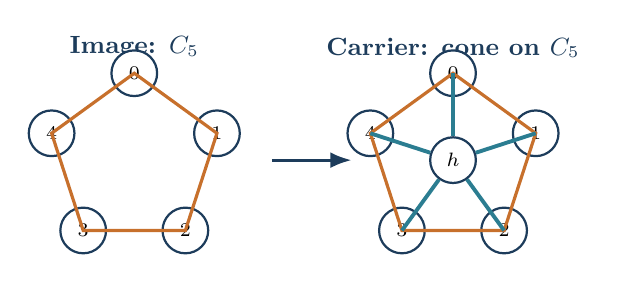
\begin{tikzpicture}[scale=.92]
\begin{scope}[shift={(-2.3,0)}]
\node[font=\small\bfseries,darkblue] at (0,1.55) {Image: \(C_5\)};
\foreach \i in {0,...,4} {\coordinate (R\i) at ({90-72*\i}:1.2);\node[vtx] at (R\i) {\(\i\)};}
\draw[source] (R0)--(R1)--(R2)--(R3)--(R4)--cycle;
\end{scope}
\draw[steparrow] (-.4,0)--(.7,0);
\begin{scope}[shift={(2.1,0)}]
\node[font=\small\bfseries,darkblue] at (0,1.55) {Carrier: cone on \(C_5\)};
\foreach \i in {0,...,4} {\coordinate (S\i) at ({90-72*\i}:1.2);\node[vtx] at (S\i) {\(\i\)};}
\draw[source] (S0)--(S1)--(S2)--(S3)--(S4)--cycle;
\node[vtx] (h) at (0,0) {\(h\)};
\foreach \i in {0,...,4}{\draw[target] (h)--(S\i);}
\end{scope}
\end{tikzpicture}
\caption{The image-induced subcomplex can be noncontractible. Adding just one target vertex produces a contractible carrier. More elaborate carriers need not have a universal vertex.}
\label{fig:extra}
\end{figure}

In \texttt{pycombtop}, the present implementation makes only a bounded attempt to find such a proof. The ordinary deletion-fold search is limited to \(24\) deletion vertices, \(18\) folds, and \(1024\) closed-neighborhood domination comparisons. When the earlier cone-image search fails, it examines at most \(36\) carriers, each on at most \(12\) vertices, allowing at most two additional vertices outside the image and at most \(64\) local \(s\)-move checks per carrier. A candidate receives an \emph{exact} verdict only after its recorded deletion folds, link images, carrier inclusion, and local dismantling moves have been independently replayed. The bounds are computational safeguards, not hypotheses of Theorem~\ref{thm:carrier}; failure to find a bounded certificate is \emph{not} a counterexample.

\section{Conclusion and further directions}
The vertex-star method is the homotopy cofiber of a specific attaching map. The contractible-carrier theorem supplies a purely combinatorial proof that this map is null: ordinary deletion folds provide a verified homotopy equivalence, while a separate certified contraction of a small induced carrier makes the composite attachment null-homotopic. In particular, the criterion avoids the false inference that vanishing homology of an image determines its homotopy type. Future improvements could use independently verified discrete Morse certificates for contractibility when neither ordinary graph folds nor bounded vertex \(s\)-dismantlings find a suitable carrier; such an extension requires a genuine contractibility certificate rather than mere acyclicity.

\begin{thebibliography}{9}
\bibitem{Hatcher2002} A. Hatcher, \emph{Algebraic Topology}, Cambridge University Press, 2002. Chapter 0, in particular Propositions 0.17 and 0.18 and Exercise 25. \url{https://pi.math.cornell.edu/~hatcher/AT/AT.pdf}.
\bibitem{Kozlov2008} D. N. Kozlov, \emph{Combinatorial Algebraic Topology}, Algorithms and Computation in Mathematics, vol.~21, Springer, 2008. \url{https://doi.org/10.1007/978-3-540-71962-5}.
\bibitem{BouletFieuxJouve2010} R. Boulet, E. Fieux, and B. Jouve, ``Simplicial simple-homotopy of flag complexes in terms of graphs,'' \emph{European J. Combin.} \textbf{31} (2010), no.~1, 161--176. \url{https://doi.org/10.1016/j.ejc.2009.05.003}.
\end{thebibliography}
\end{document}
